\chapter{Tecnologie}

\section{Docker}

Docker è diventato negli anni il sistema più popolare per gestire la virtualizzazione basata su container. In realtà, la sua value proposition è legata alla possibilità di poter lanciare una applicazione ovunque, con la garanzia che questa funzioni sempre. L'analogia con i container nel mondo reale è diretta: i container utilizzati nel commercio, possono essere adattati indipendemente dall'ambiente di trasporto. Allo stesso modo l'applicazione che viene eseguita, funzionerà indipendemente dall'ambiente di esecuzione, qualsiasi sistema operativo esso sia, con l'unica limitazione sull'instruction set per cui è stata generata la build. Possono anche essere visti come macchine virtuali leggere, perché riescono a garantire le stesse caratteristiche di quelle tradizionali, ma con un overhead minore, sia in termini di efficienza nell'esecuzione, che di spazio occupato. 

\begin{figure}[htbp]
    \centering
    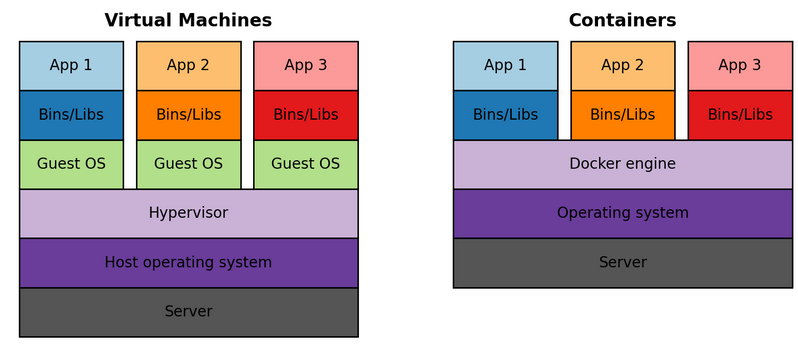
\includegraphics[width=0.8\textwidth]{figures/containers-and-vms.png}
    \caption{Confronto tra macchine virtuali tradizionali e containers. Essi vengono eseguiti direttamente sul sistema operativo dell'host, senza la necessità di chiamate di sistema multiple. Vengono impacchettate solo le librerie necessarie nell'immagine di base fornita al container.}
    \label{fig:virt-tech}
\end{figure}

Nella pratica esistono due definizioni secondo chi è l'utilizzatore di questa tecnologia: se si parla di gestione di una infrastruttura, allora l'attenzione è spostata verso la virtualizzazione, mentre se il focus è relativo alle applicazioni allora si può vedere Docker come una tecnologia orientata alla portabilità. In generale, le macchine virtuali devono garantire un serie di proprietà per poter essere definite tali, che sono:

\begin{itemize}
	\item \textbf{consolidamento}: inizialmente ciascuna applicazione veniva eseguita su una macchina distinta, rendendo l'utilizzo delle risorse inefficiente. La virtualizzazione ha permesso di superare questa limitazione, con l'esecuzione di software differenti all'interno della stessa macchina.
	\item \textbf{isolamento}: questa proprietà consente ad ogni applicazione di vedere l'ambiente come se fosse una macchina a sé stante, nonostante il consolidamento. I sistemi operativi offrono funzionalità di isolamento base come l'astrazione dello spazio di indirizzamento di un processo, ma questo non è sufficiente per una applicazione self-contained. Diversi applicativi infatti possono interferire tra di loro già solo nell'utilizzo della memoria, nel caso di sovra-allocazioni, portando ad un degrado delle prestazioni o al crash(verifica). Lo stesso ragionamento si può applicare anche per la gestione della cpu, della rete e del filesystem che all'interno di un sistema operativo sono risorse completamente condivise tra processi. 
	\item \textbf{flessibilità}: il controllo dei container è molto semplice in quanto docker prevede dei comandi standard per la loro gestione, come l'avvio, la pausa e lo stop. Gli orchestratori giocano un ruolo fondamentale per riallocare i container in nodi diversi dell'infrastruttura, per esempio in caso di manutenzione o sovraccarico. Questo processo avviene senza particolari overhead, in quanto i container, a differenza delle macchine virtuali tradizionali hanno dei tempi di attivazione molto bassi.
	\item \textbf{portabilità}: come già visto, i container possono essere avviati in qualsiasi piattaforma, indipendemente dal sistema operativo, dall'hardware, dalle librerie necessarie e dalle loro versioni. Questo comporta un grande vantaggio anche nell'uso di linguaggi di programmazione di basso livello quando l'efficienza è fondamentale. Linguaggi come Java, ad esempio, si servono di macchine virtuali per poter garantire la portabilità del codice, ma il tempo di esecuzione aumenta notevolmente. 
\end{itemize}

L'implementazione dei container è stata possibile grazie a due elementi presenti all'interno dei sistemi operativi: namespaces e control groups(cgroups). Si tratta di features che inizialmente non erano state pensate per la virtualizzazione, ma solo nell'ottica di avere dei processi isolati. Non si è quindi arrivati subito alla definizione di container, ma ci sono state delle tappe risolutive di diversi problemi che gli sviluppatori avevano all'inizio degli anni 2000. I namespaces permettevano la gestione della visibilità relativa alle risorse per ogni processo, mentre i cgroups servivano a limitare l'utilizzo di quanto allocato. Nel secondo caso, esistevano già dei meccanismi di questo tipo all'interno del kernel Linux (e.g. cpulimit, nice), ma non erano centralizzati e potevano essere applicati solo a singoli processi. L'evoluzione dei cgroups è fondamentalmente quella di estendere il tutto ad un gruppo di task in maniera modulare, con la possibilità di definire delle gerarchie nella gestione delle risorse. Le tecnologie basate su container come Docker hanno integrato questi meccanismi nel loro layer di virtualizzazione, in modo tale da fornire delle primitive di alto livello per la gestione dei container, che altrimenti con le precedenti astrazioni sarebbero accessibili solo ad utenti esperti, ed in ogni caso inclini ad errori a causa della complessità di utilizzo. 

Docker presenta infine una particolarità a livello di filesystem: rispetto alle macchine virtuali tradizionali o container LXC, che sfruttano un filesystem in senso stretto, questa tecnologia utilizza il concetto di Union Filesystem. Si tratta di un sistema che combina diversi filesystem restituendo logicamente un'unica struttura. Nell'implementazione di Docker, lo Union Filesystem si presenta come una gerarchia di strati, tutti in sola lettura, a ne cui viene aggiunto uno scrivibile al lancio del container. Questo meccanismo permette la condivisione della stessa immagine di base, evitando allo stesso tempo di dover duplicare lo spazio di memoria e che modifiche da parte di una macchina possano influenzare ciò che vedono gli altri container basati sulla stessa istanza, attuando così un primo livello di isolamento (quello più generale con l'host viene sempre implementato attraverso i namespaces). 

\begin{figure}[htbp]
    \centering
    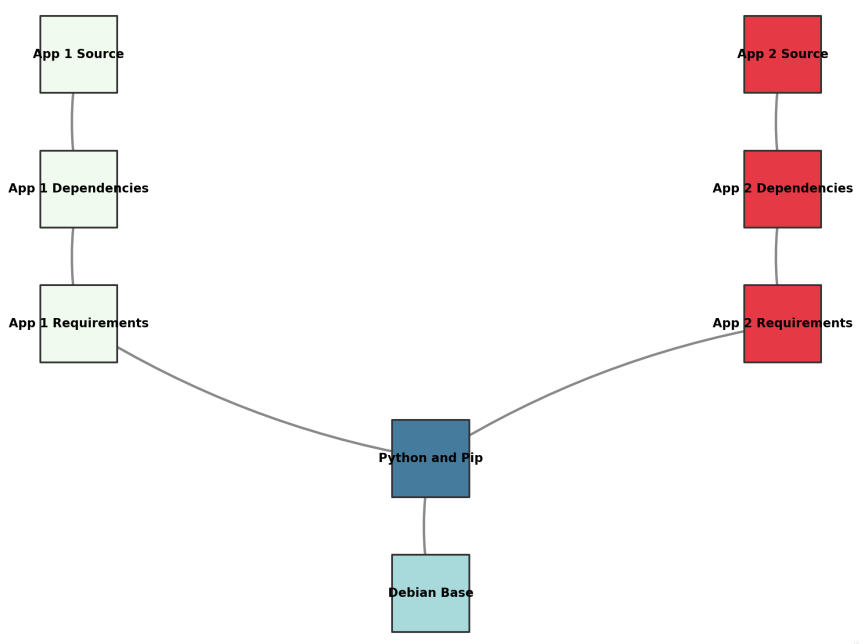
\includegraphics[width=0.65\textwidth]{figures/docker-image-layers.png}
    \caption{Esempio di condivisione di layers in Docker. Le due immagini risultanti hanno la stesso sistema di base, condividendo lo stesso ambiente (Debian) e runtime (Python).}
    \label{fig:image-layers}
\end{figure}

La realizzazione pratica di questa funzionalità è possibile grazie al concetto di copy-on-write, già utilizzato nella creazione dei processi. In questo caso il funzionamento è analogo, ma si applica a livello di memoria secondaria. Ogni modifica all'immagine di base, attraverso il layer in scrittura di più alto livello, è ciò che viene salvato. Non si apportano modifiche all'intera memoria: in pratica è un meccanismo basato sulle differenze. Una volta che si esegue il commit di un'immagine, gli strati vengono congelati e ne formano una nuova. Al livello dell'utilizzatore questo sistema si rivela molto utile perché si possono comporre nuove immagini impilando nuovi layer a quelli già esistenti, senza preoccuparsi dei livelli sottostanti, perché grazie alla portabilità il loro funzionamento è garantito. La composizione non è l'unica proprietà interessante che emerge da questa architettura, ma anche modularità, riutilizzo ed efficienza. Quest'ultima è importante sia in termini di spazio, perché come già visto i layer inferiori vengono condivisi, sia in termini di tempo. Quando si costruisce una nuova immagine, infatti, verranno aggiunti o scaricati solo gli strati di più alto livello per la generazione della nuova immagine, invece di dover ri-eseguire l'operazione ogni volta.
  	
\section{MQTT} %mancano definizione esplicita del protocollo, ma emergono nelle responsabilità del broker; subscribe, unsubscribe
Message Queue Telemetry Transport (MQTT) è un protocollo orientato ai messaggi, basato su TCP, il cui obiettivo è quello di fornire un protocollo leggero, per dispositivi con risorse limitate e connessioni instabili. Il formato dei dati infatti è semplice ed è pensato per essere affidabile e fault-tolerant. Proprio per le sue caratteristiche, con il tempo è diventanto uno standard nelle le applicazioni IoT, ad esempio monitoraggio remoto e raccolta di dati in industria, domotica e ambiente. MQTT si basa su un'architettura publish-subscribe. Ciò permette di disaccoppiare l'invio dei messaggi tra produttori e consumatori, attraverso un broker. Si tratta di un metodo di comunicazione indiretto, in quanto per chi pubblica non è necessario conoscere la destinazione, come invece avviene nelle architetture client-server. Il funzionamento è analogo a quello delle newsletter. Quando un utente è interessato ad un certo argomento, lascia il proprio indirizzo email, in modo tale da ricevere aggiornamenti. Analogamente in un sistema publish-subscribe le entità che devono ricevere determinati messaggi da un publisher, si iscrivono ad un canale. 

\begin{figure}[htbp]
    \centering
    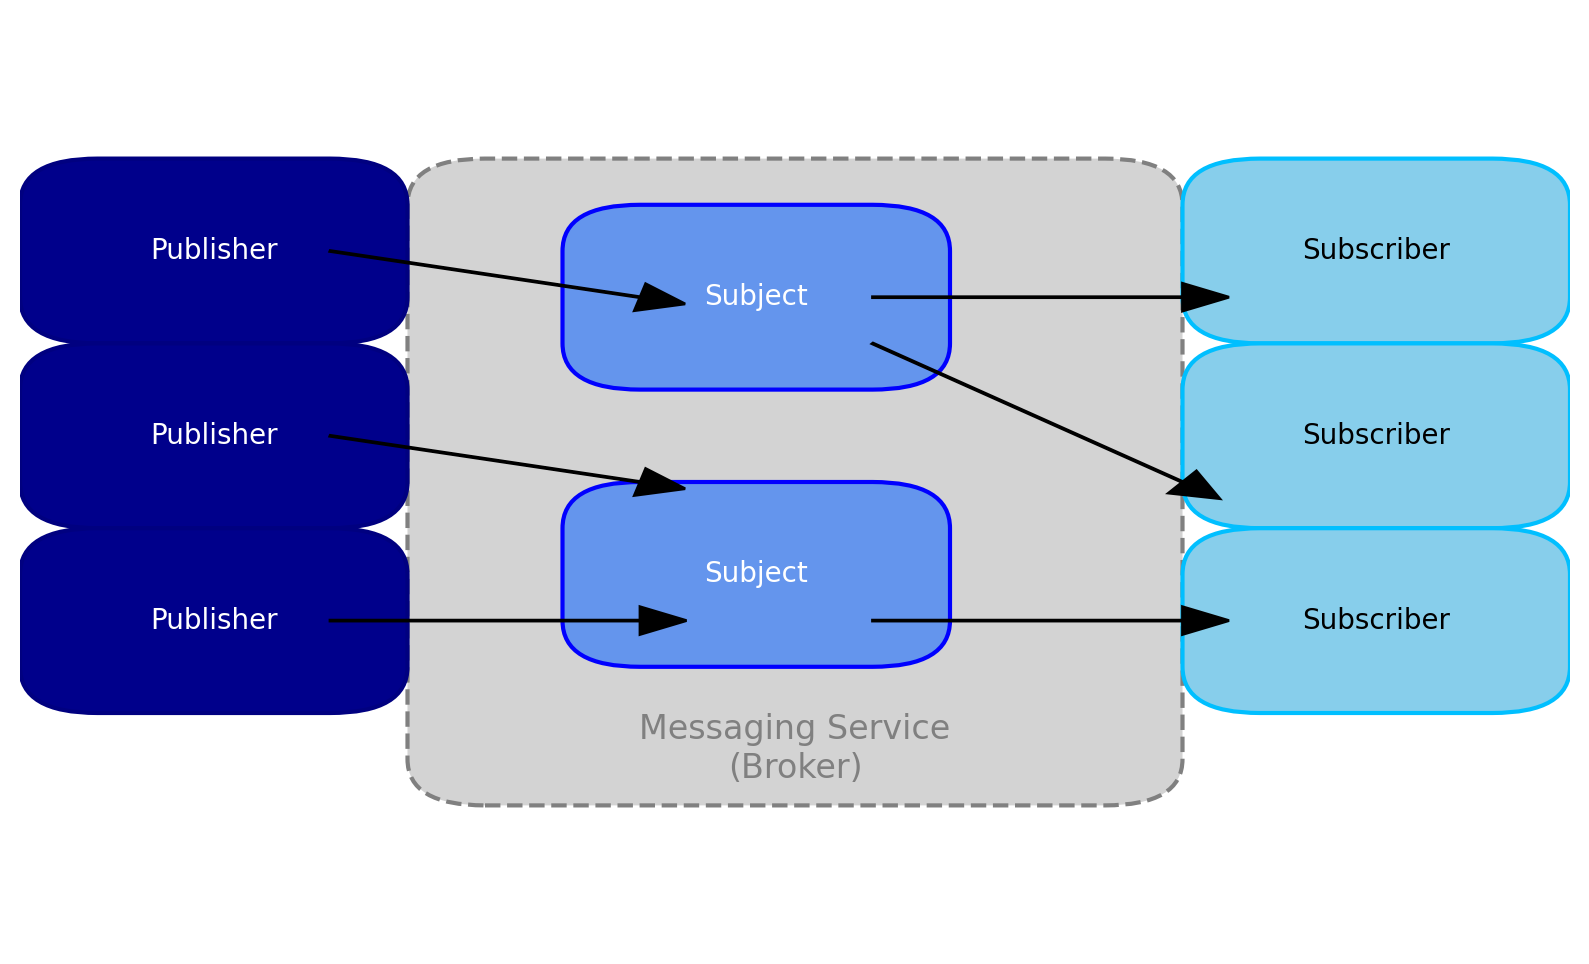
\includegraphics[width=0.65\textwidth]{figures/pub-sub-arch.png}
    \caption{Schema architettura publish-subscriber.}
    \label{fig:pub-sub}
\end{figure}

Oltre al disaccoppiamento, questo tipo di pattern fornisce ulteriori vantaggi. E' possibile aggiungere nuovi publisher o subscriber senza dover modificare la logica esistente, il che rende l'architettura facilmente scalabile. Si tratta di uno dei motivi per cui il cloud riesce a gestire facilmente milioni di messaggi in un breve intervallo di tempo ed avere migliaia di publishers. Inoltre ogni parte del sistema non dipende dalle altre, favorendo la comunicazione asincrona, poiché nessun publisher deve aspettare per l'invio di nuovi messaggi prima che i consumatori finiscano. Allo stesso modo i consumatori non devono attendere che altri ricevano i messaggi per poter proseguire con l'elaborazione delle proprie informazioni. Questo tipo di pattern viene implementato in tanti sistemi come quelli delle notifiche push nelle applicazioni mobili, nei servizi gestiti del cloud ed infine nei sistemi IoT, attraverso il protocollo MQTT, focus dei paragrafi successivi. In questo contesto, le unità di interesse vengono descritte come topic. Essi sono univocamente definiti all'interno dei broker attraverso una struttura gerarchica che ricorda i path nelle URI. Ad esempio, un topic può essere dichiarato come: \texttt{factory/floor/sensor1}. Non esiste un meccanismo esplicito di creazione dei topic, ma vengono definiti contestualmente alla pubblicazione di un messaggio.

Il broker ha la responsabilità di connettere, se autorizzati, i diversi client della rete, di tenere traccia dello stato di connessioni precedenti e di filtrare i dati in arrivo dai publisher. Per il discorso di efficienza previsto da questo protocollo, infatti, devono essere distribuiti solo i pacchetti necessari al funzionamento del sistema, e quindi la capacità di filtro è un elemento fondamentale. In particolare, esistono diverse tipologie di controllo dei pacchetti in transito. Quello più importante è il topic filter, dove un messaggio deve contenere necessariamente un topic nell'header, e sarà compito del broker ritrasmetterlo o ignorarlo in base a come è stata implementata la sua logica. In generale i filtri vengono usati per riferirsi ad un insieme di topic, sfruttando due tipologie di wildcards. Si utilizza il segno "+" per indicare un intero livello nella gerarchia del path definito dal topic. Ad esempio \texttt{factory/+/sensor1} serve per tutti i sensor1 nei diversi piani di una fabbrica. Il secondo simbolo, cioè "\#" si riferisce ad una intera sottogerarchia nel path. \texttt{factory/\#} e \texttt{factory/first/\#} filtrano rispettivamente tutti i messaggi provenienti dalla fabbrica e quelli provenienti dal primo piano di un complesso industriale. 

MQTT è un protocollo progettato con l'affidabilità in mente: in base al contesto (hardware, banda, latenza) e al tipo di applicazione, fornisce diversi livelli di Quality of Service(QoS):

\begin{itemize}
	\item \textbf{QoS0}: modalità di funzionamento default in MQTT, se non specificato. I messaggi vengono inviati con una logica fire-and-forget, senza la garanzia che il processo vada a buon fine. Il publisher o il broker inviano i messaggi senza alcun tipo di risposta da parte di un subscriber. Non ci sono ulteriori garanzie oltre a quelle fornite dal protocollo TCP.
	\item \textbf{QoS1}: garantisce che il messaggio venga inviato almeno una volta. Questo meccanismo si basa su messaggi di acknowledgment provenienti dal ricevente, per cui se non arriva nessuna risposta, il messaggio deve essere ritrasmesso.
	\item \textbf{QoS2}: si tratta del livello di qualità più alto. Il messaggio viene inviato una sola volta, grazie ad una serie di messaggi di controllo generati dalle entità in gioco. Può essere visto come un acknowledgement incrociato tra publisher e ricevente. Quello che avviene in più rispetto a QoS1 è l'invio dei pacchetti publish-realease per indicare il rilascio del messaggio dalla memoria del publisher, e publish-complete da parte del ricevente per chiudere la comunicazione. In questo modo alla fine del processo il messaggio è stato inviato e gli attori in gioco sono totalmente sincronizzati dal punto di vista della ricezione.   
\end{itemize}

\begin{figure}[htbp]
    \centering
    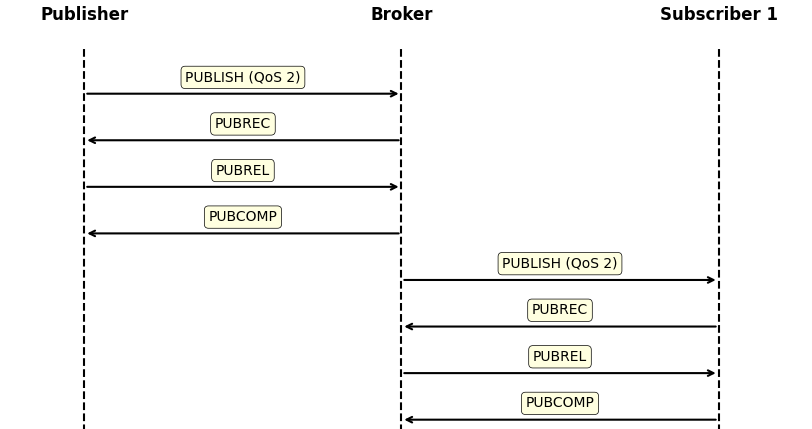
\includegraphics[width=0.9\textwidth]{figures/qos2.png}
    \caption{Flusso pacchetti di controllo per QoS2. I livelli più semplici funzionano in maniera simile, con un numero di pacchetti inferiore. Si può notare come il disacoppiamento fornito dal broker faciliti lo scambio dei messaggi.}
    \label{fig:qos2}
\end{figure}





Il QoS viene negoziato al momento della connessione con il broker, ed in base alle sue capacità può essere dinamicamente modificato in un secondo momento. Nell'affrontare il concetto di qualità di servizio, si è visto quindi il funzionamento della publish da parte di un client, ma esistono altri tipi di operazioni in questo pattern, cioè subscribe, unsubscribe e ping. In particolare quest'ultimo risulta fondamentale per l'implementazione del Last Will and Testament(LWT), un metodo per comunicare la disconnessione di un publisher all'interno della topologia. LWT è un messaggio contente il topic, il QoS e un payload da inoltrare a tutti i subscriber che fino a quel momento ricevevano le notifiche. Questo pacchetto viene fornito nel momento in cui un client si connette per la prima volta al broker, prima che inizi l'invio effettivo dei dati per gli altri client. Se attraverso delle operazioni di ping, impostate con un certo timer, una delle due parti non riceve risposta, allora si assume esserci stata una disconnessione. A quel punto, se è il client ad essere offline, il broker invierà il Will ai subscribers.

Un'ultima caratteristica importante per il funzionamento di MQTT, è la persistenza. Il broker mantiene le informazioni di sessione per i client disconnessi, in modo tale da riottenere facilmente le iscrizioni ai topic e i messaggi in coda che non avevano ricevuto (se si tratta di QoS1 e QoS2, pensati come già visto per la trasmissione affidabile). Inoltre, i publisher possono impostare un flag RETAINED nei messaggi, in modo tale che venga salvati in maniera indefinita nel broker. L'obiettivo di questa funzionalità è garantire l'invio di un determinato messaggio ad un client indipendetemente dal momento della sua iscrizione al topic.  

\section{RTSP}
\section{Amazon Web Services}
\subsection{Infrastructure as Code}
\subsection{Serverless}
\subsection{Iam Policy}
\subsection{Kinesis Video Streams}
\subsection{AWS Iot Core e Greengrass}
\section{Apache Flink}
\section{GStreamer}



